\documentclass[journal,final]{new-aiaa}
\usepackage[utf8]{inputenc}
\usepackage{color}
\usepackage{algorithm}
\usepackage[noend]{algpseudocode}
\usepackage{graphicx}
\usepackage{amsmath}
\usepackage[version=4]{mhchem}
\usepackage{siunitx}
\usepackage{longtable,tabularx}
\setlength\LTleft{0pt}

\newcommand{\A}{\mathbf{A}}
\newcommand{\B}{\mathbf{B}}
\newcommand{\C}{\mathbf{C}}
\newcommand{\D}{\mathbf{D}}
\newcommand{\E}{\mathbf{E}}
\newcommand{\F}{\mathbf{F}}
\newcommand{\G}{\mathbf{G}}
\newcommand{\HH}{\mathbf{H}}
\newcommand{\I}{\mathbf{I}}
\newcommand{\J}{\mathbf{J}}
\newcommand{\K}{\mathbf{K}}
\newcommand{\LL}{\mathbf{L}}
\newcommand{\PP}{\mathbf{P}}
\newcommand{\R}{\mathbf{R}}
\newcommand{\U}{\mathbf{U}}
\newcommand{\W}{\mathbf{W}}
\newcommand{\w}{\mathbf{w}}

\newcommand{\uu}{\mathbf{u}}
\newcommand{\n}{\mathbf{n}}
\newcommand{\rr}{\mathbf{r}}
\newcommand{\s}{\mathbf{s}}
\newcommand{\e}{\mathbf{e}}
\newcommand{\ddd}{\mathbf{d}}
\newcommand{\f}{\mathbf{f}}
\newcommand{\T}{\mathbf{T}}
\newcommand{\x}{\mathbf{x}}
\newcommand{\y}{\mathbf{y}}
\newcommand{\ttt}{\mathbf{t}}
\newcommand{\bb}{\mathbf{b}}

\newcommand{\vv}{\mathbf{v}}
\newcommand{\boldalpha}{\boldsymbol{\alpha}}


\newcommand{\df}[2]{\dfrac{\partial#1}{\partial#2}}
%\newcommand{\dd}[3]{\dfrac{\partial^2#1}{\partial#2 \partial#3}}
\newcommand{\dd}[3]{{\partial^2#1}/{\partial#2 \partial#3}}
\newcommand{\ff}[2]{\dfrac{d#1}{d#2}}
\newcommand{\ds}[2]{\dfrac{\partial^2#1}{\partial#2^2}}
\newcommand{\dn}[3]{\dfrac{\partial^{#1}#2}{\partial#2^{#1}}}

\newcommand{\dis}{\displaystyle}

\newcommand{\npo}{n\!\!+\!\!1}

\newcommand{\grad}{\textrm{grad\,}}
\newcommand{\Div}{\textrm{div\,}}

\newcommand{\half}{\frac{1}{2}}
\newcommand{\third}{\frac{1}{3}}
\newcommand{\quarter}{\frac{1}{4}}

\newcommand{\Atv}{\A^{\!T}\!v}
\newcommand{\Au}{\A u}
\newcommand{\RK}{R-K\@\xspace}
\newcommand{\vtf}{v^T\!f}
\newcommand{\gtu}{g^T\!u}

\newcommand{\degr}{^{\circ}}
\newcommand{\logt}{\log_{10}}
\newcommand{\dsps}{\displaystyle\strut}

\newcommand{\ind}{\phantom{\bf do}}

\graphicspath{{./pic/}}

\title{Rotating flow instability prediction using eigenvalue analysis}
\author[1]{Shenren Xu	
\footnote{ Corresponding author, email address: shenren\_xu@nwpu.edu.cn}}
\affil[1]{School of Power and Energy, 
	Northwestern Polytechnical University, Xi'an, 710072, China}
%\author[1]{Xiuquan Huang}
%\author[1]{Dingxi Wang}

\begin{document}
\maketitle

\begin{abstract}
The compression system in turbomachines, e.g.,  aircraft engines and gas turbines,
when operating under off-design conditions, exhibits self-excited unsteady phenomena
such as surge, rotating stall and rotating instability, leading to performance deterioration
and/or structural damages. Inability to accurately predict when such flow instability occurs
limits the development of high performance compression system. In this paper,
an eigenvalue problem is solver to (1) predict the linear stability and (2) find the
destabilizing eigenmode for a classical 
commonly seen for turbomachines operating at near stall conditions. The eigenvalue
analysis is fully based on the steady state three-dimensional Reynods-averaged
Navier-Stokes equations and thus the stability boundary is fully consistent with
the one that is predicted by the time-accurate flow simulation, i.e., URANS, but
two to three times faster.
The method is applied to the computation of stability boundary of
(i) the laminar flow around a two-dimensional circular cylinder,
(ii) the flow around a quasi-three-dimensional compressor anuular cascade, 
and 
(iii) flow around a three-dimensional compressor rotor.
The method developed here has the potential to revive
the once-popular eigenvalue method for prediction rotating stall and surge, which
was based on lower-fidelity flow models and provide industry with tools to
accurately predict the stall line in the early design stage.
\end{abstract}

%\section*{Nomenclature}
%{\renewcommand\arraystretch{1.0}
%\noindent\begin{longtable*}{@{}l @{\quad=\quad} l@{}}
%$c_v,c_p$   & specific heat \\
%$e$     & internal energy\\
%$E$     & total energy\\
%
%$\partial \Omega_r$& boundary of $\Omega_r$
%\end{longtable*}}

\section{{\color{red}Todo list}}

\begin{itemize}
	\item  {\color{red} Investigate the fouriour spectrum
		of the circumferential signal of the eigenvectors and
		interpret the various frequency components.}
	\item {\color{red} Investigate the influence of the axial
		location where the circumferential signal is taken.}
	\item {\color{red} Label relevant eigenmodes with NDs.}
	\item {\color{red} Compare unstable modes with URANS.}
\end{itemize}


\section{Introduction}
Rotating stall and rotating instability has been studied extensively
both experimentally and numerically. However, previous numerical
investigations mainly focused on using time-dependent unsteady
flow analysis using a fraction of the annulus. Flow physics for
the destablization mechanism has been investigated in depth
but little insight has been gained. Eigenvalue analysis is a powerful
yet inexpensive tool to probe the flow near the critical condition,
revealing rich flow physics with cost comparable to a steady state
analysis. In this work, we demonstrate that using eigenvalue analysis
based on a whole-annulus steady state solution, the linear stablity
demarcation point can be pinpointed with the cost of a few steady
state analysis, and a full-annulus time-accurate unsteady calculation
can thus be avoid. This methodology enables a quick parameter
study to investigate the various rotating flow instability phenomenon
such as rotating stall and rotating instability.

\section{The nonlinear flow solver}
%The nonlinear flow solver used in this work is NutsCFD, an unstructured
%finite volume Reynolds-averaged Navier--Stokes solver capable of dealing
%with rotating frame reference and periodic boundary conditions.
%The solver features the use of a noval Newton--Krylov algorithm,
%which significantly enhances the efficiency and robsutness when
%computing turbomachinery flows at off-design conditions.
%Details of the NK algorithm can be found in~\cite{123} and
%only general information of the solver theory is provided below.

\subsection{Governing equations}
%The integral form of the governing equations in a
%relative frame of reference with an angular
%velocity of $\boldsymbol \omega$ is
%\begin{equation*}
%\dfrac{d}{dt}\int_{\Omega_r} \W dV
%+\oint_{\partial \Omega_r} (\F^r_c-\F_v)dS
%+\int_{\Omega_r}\F_\omega dS
%=0,
%\label{governing}
%\end{equation*}
%where $\W$ are %is
%the conservative variables
%$\left[\rho,~\rho\uu,~\rho E\right]^T$.
%The absolute and relative convective fluxes,
%$\F_c$ and $\F^r_c$,
%the viscous flux $\F_v$,
%and the additional flux due
%to rotation, $\F_\omega$,
%are defined as %follows
%\begin{equation*}
%\F_c=
%\left [ 
%\begin{array}{c}
%\rho \uu \cdot \n\\
%\rho \uu \uu\cdot \n +  p\n\\
%\rho H \uu \cdot \n
%\end{array}
%\right],
%\text{~~}
%\F^r_c=
%%\left [ 
%%\begin{array}{c}
%%\rho \uu \cdot \n\\
%%\rho \uu \uu\cdot \n +  p\n\\
%%\rho H \uu \cdot \n
%%\end{array}
%%\right]
%\F_c
%-
%(\uu_{rot}\cdot \n) 
%\left [ 
%\begin{array}{c}
%\rho\\
%\rho \uu\\
%\rho E
%\end{array}
%\right ]
%,\text{~~}
%\F_v=
%\left [ 
%\begin{array}{c}
%0\\
%\tau \cdot \n\\
%\uu \cdot \tau \cdot \n + \kappa \n \cdot \nabla T
%\end{array}
%\right ],\text{~~}
%\F_\omega=
%\left [ 
%\begin{array}{c}
%0\\
%\rho {\boldsymbol{\omega}} \times \uu\\
%0
%\end{array}
%\right ],
%\end{equation*}
%with $\uu_{rot}={\boldsymbol \omega} \times \x$.


\subsection{Spatial discretization}
%The governing equations are discretized using the
%method of lines and thus the spatial and temporal
%discretizations can be treated separately.
%The governing equations for the
%steady state solution $\W$ is
%\begin{equation}
%\R(\W)={\bf 0},
%\label{nonlinear}
%\end{equation}
%where $\R$ is the sum of fluxes and source terms
%associated with each control volume. Suppose control
%volume %node
%$i$ has $N$ flux faces with
%area $S_{ik}$ for
%$k=1,2,...,N$.
%$R_i$ then is 
%\begin{equation*}
%R_i(\W)=\sum^{N}_{k=1} (\F^r_c-\F_v)S_{ik}+\F_{\omega} V_i,
%\end{equation*}
%where $V_i$ denotes the volume.
%
%Turbulence is modelled using the negative Spalart--Allmaras
%(SA-neg) model~\cite{allmaras2012modifications}.
%Compared to the original SA model~\cite{allmaras2012modifications},
%this avoids the clipping of the turbulent variable
%to a non-negative value which potentially
%prevents the full convergence of the nonlinear solver.
%The turbulence equation is discretized using
%the first-order accurate upwind
%scheme~\cite{langer2014agglomeration}.
%
%\subsection{Temporal discretization}
%The time-marching of the nonlinear equation is
%based on Newton's method.
%Equation~\eqref{nonlinear} is solved by iteratively updating
%the solution as
%\begin{equation*}
%  \W^{n+1}=\W^n+ \Delta \W
%  \label{newtonTransient}
%\end{equation*}
%until convergence is reached, i.e., $\|\R(\W)\|=0$,
%where $\Delta \W$ is the solution to the linear 
%system of equations
%\begin{equation*}
%  \df{\R}{\W}\Delta \W = -\R(\W^n) 
%\end{equation*}
%The exact Jacobian matrix is computed with the
%help of automatic differentiation tool
%Tapenade~\cite{Tapenade}
%and the graph coloring package
%Colpack~\cite{gebremedhin2013colpack}.
%The sparse linear system of equations arising
%from the linearization of $\R$ is solved with
%the Krylov-subspace solver, GMRES, with
%incomplete LU factorization (ILU) as the
%preconditioner. The overall algorithm
%is the Newton--Krylov (NK) method. Special care is
%taken to handle the periodic boundary condition
%when simulating flows in a single passage.

\subsection{Temporal discretization}


\section{Global linear stability analysis}
For a nonlinear dynamic system, e.g., the discretised NS equation, using
the method of lines,
the governing equation is
\begin{equation}
\dfrac{d\uu}{dt}=-\R(\uu)
\end{equation}
where $\uu$ is the time-varying flow variable and $\R(\uu)$ is the nonlinear
residual representating the spatial discretization.
Assuming a steady state solution $\uu_0$ (equilibrium point of the dynamic system)
exists, and the time-varying flwo variable can be decomposed as the
steady and the unsteady part 
\begin{equation}
\uu:=\uu_0 + \tilde \uu
\end{equation}
and the governing equation becomes
\begin{equation}
\dfrac{d \tilde \uu}{dt}=A \tilde \uu
\end{equation}
where $A$ is the negative Jacobian $A:=-\df{\R}{\uu}$.

In order to use the eigen model decomposition approach, suppose
the system matrix has right eigenvectors $\{\vv_i, \vv_2, ..., \vv_N\}$,
which forms the matrix $V$ as its colum vectors. Matrix $A$ can then
be factorized as 
\begin{equation}
A=V\Lambda V^{-1}
\end{equation}
where the diagonal matrix $\Lambda$ has the eigenvalues on the matrix $A$
as its diagonal elements.
Decomposing the unsteady part $\tilde \uu$ in the eigen modal space,
it can be expressed as a linear combination of all eigenvectors with
coordinates $\eta$
\begin{equation}
\tilde \uu = V \eta
\end{equation}
Substituting the $\tilde \uu$ in the governing equation using the eigen modal
decomposition, it becomes
\begin{equation}
\dfrac{d \eta}{dt}= \Lambda \eta
\end{equation}
Different from the original coupled system, all variables are decoupled now and it
can be written as
\begin{equation}
\dfrac{d \eta_i}{dt}= \lambda_i \eta_i  ~~~\forall i
\end{equation}
For the linear system to be stable, the sufficient and necessary condition is
that all eigenvalues has a negative real part, i.e., real$(\lambda_i), \forall i$.

\subsection{Numerical implementation}
In practice, performing the global linear stability analysis as described above
is a standard procedure involving three steps:
\begin{itemize}
	\item Find an equilirium point (converging to steady state solution);
	\item Linearize the nonlinear residual and form the Jacobian matrix;
	\item Calculate the eigenvalue with the largest real part.
\end{itemize}

\subsection{Time-domain unsteady approach}
\subsection{Eigenvalue approach}
\section{Eigenvalue analysis for large sparse matrices}

\section{Results}
\label{results}

\subsection{Laminar flow around a two-dimensional circular cylinder}
Eigenvalue analysis is performed for the canonical case of the
laminar flow around a circular cylinder with the Reynolds number in
the range between 40 and 100. The computational domain is a
circular cylinder centered at the origin with a diameter of $D=10^{-5}$
and the farfield is a circle with a diameter of $100D$. The left half of
the outer circle is set to 'farfield' boundary condition with a incoming
flow of Mach 0.2 in the x-direction, a static pressure of $101325~Pa$ and
and a temperature of $288.15~K$.
The right half ot he circle is set to 'pressure-outlet' boundary condition,
with a constant pressure of $101325~Pa$.
The computational domain is meshed with quadrilateral elements,
with a total of 29600 grid points. The density is $1.225~kg/m^3$.
The dynamic viscosity is varied in order to achieve a particular Reynolds number.

\subsubsection{Steady state calculation}
The steady state flow is obtained by either using an implicit solution method in
Fluent (version 19.2) or by resorting to the Newton-Krylov algorithm in NutsCFD,
despite the fact that the flow is physically unsteady under this condition. The
Mach number contour of the NutsCFD calculation is shown in Fig.~\ref{fig:cyl-re55}.

\begin{figure}[htb]
	\centering   
	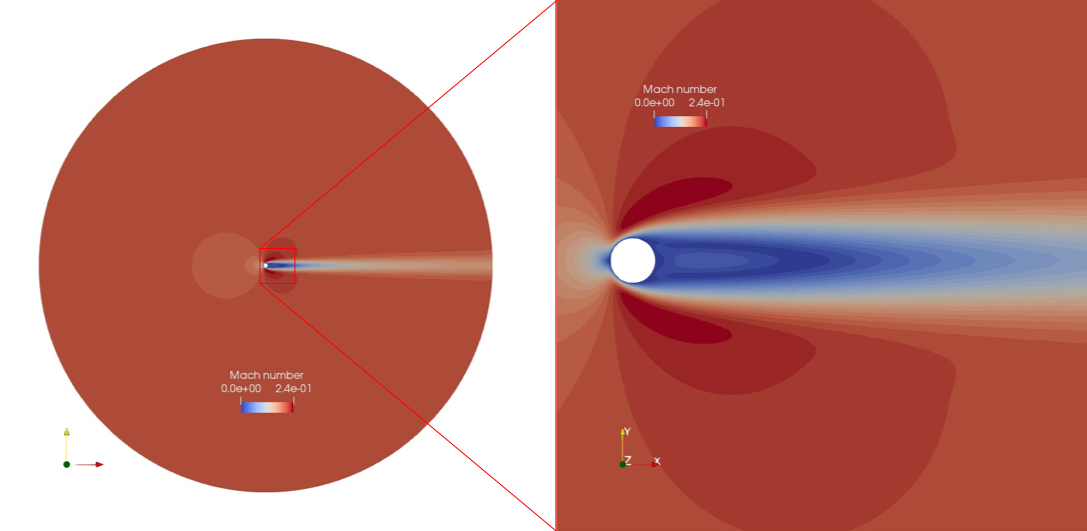
\includegraphics[width=0.75\textwidth]{pic/cylinder-std.png}
	\caption{Mach number contour plot of the calculation results by NutsCFD for Re = 55.}
	\label{fig:cyl-re55}
\end{figure}

To compare the Fluent and NutsCFD results quantitatively, the velocity-x
behind the cylinder as well as the pressure coefficient along the cylinder
surface are compared in Fig.~\ref{fig:cyl-re55-u-cp} and very good agreement
can be found.
\begin{figure}[htb]
	\centering   
	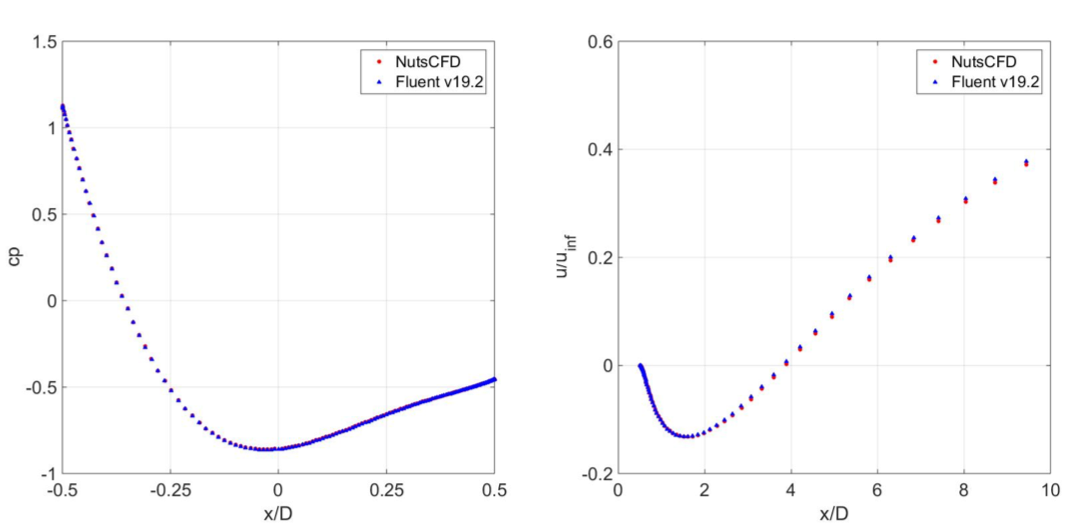
\includegraphics[width=0.75\textwidth]{pic/cylinder-std-compare.png}
	\caption{Comparison between Fluent and NutsCFD calculation results for
		velocity-x along the center line behind the cylinder (left) and pressure
		coefficient along the cylinder surface (right).}
		\label{fig:cyl-re55-u-cp}
\end{figure}

\subsubsection{Unsteady calculation}
Experimental results show that the laminar flow around the cylinder
becomes unsteady for Re above a critical value (around 47). To study
this phenomenon, unsteady flow calculation for $Re=55$ and $Re=40$
are performed using Fluent. First, for both conditions, a steady
state flow solution is obtained by converged the residual to machine error.
For $Re=55$, the unsteady simulation is run with the steady state
as initial condition. A BDF2 second-order implicit dual-time-stepping
method is used with the physical time step set to $10^{-8} sec$, that is, $0.01 ms$,
and
the inner loop is solved with a CFL of 1000 and maximum 5 iterations.
Roughly two orders of magnitude of residual drop is achieved for the
inner loop. From Fig.~\ref{fig:cyl-re40-re55-uns}, it can be seen
that after around $100 ms$, the lift coefficient starts to grow and
eventually reaches a saturated limit cycle at around $130 ms$.
On the contrary, running unsteady simulation with a fully converged
steady state for $Re=40$ does not lead to unsteadiness. To probe
the flow at $Re=40$ further, a disturbance is introduced into the
flow from the farfield by setting the incoming flow direction to vertical
for one time step and switching it back to the horizontal direction,
and then continue the unsteady run. The lift coefficient shows a
transient response but eventually slowly delays to zero. These
two sets of lift coefficient signals are plotted in Fig.~\ref{fig:cyl-re40-re55-uns}
in both linear and logrithm scales. The logrithmic plot on the right
clearly shows an exponential growth and decay for $Re=55$ and $Re=40$,
respectively.

{\color{red} The growth and decay rate for both conditions can be extracted
	from the time signal and then be compared to the eigenvalue analysis
	results.}


{\color{red} The same unsteady simulation is not performed in NutsCFD
	as the code is slower than fluent and in the meantime, it is believed
	that the unsteady response between the two solvers will be very similar,
	based on the comparison of the steady state solutions.}


\begin{figure}[htb]
	\centering   
	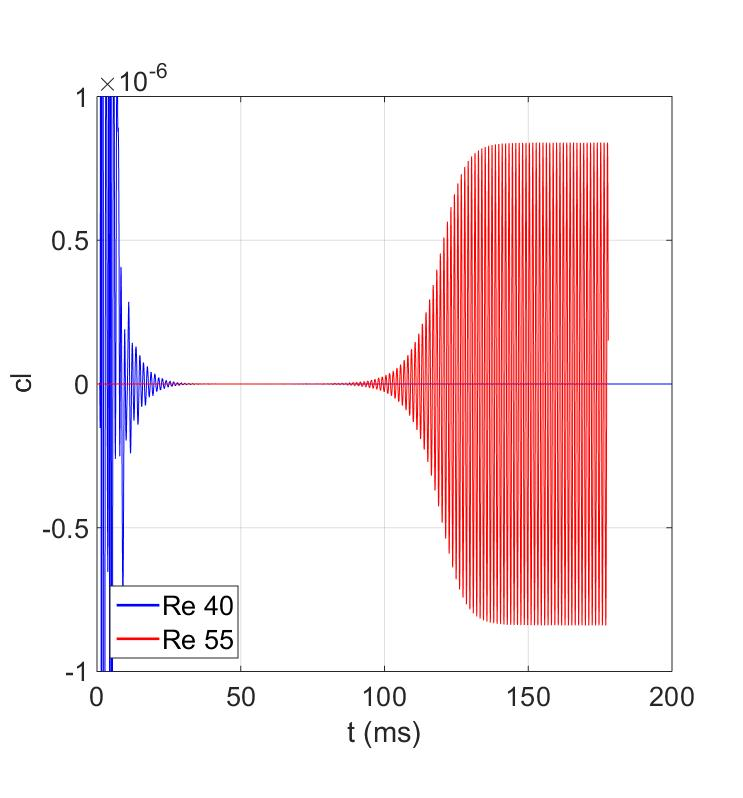
\includegraphics[width=0.49\textwidth]{pic/cl-linear.jpg}	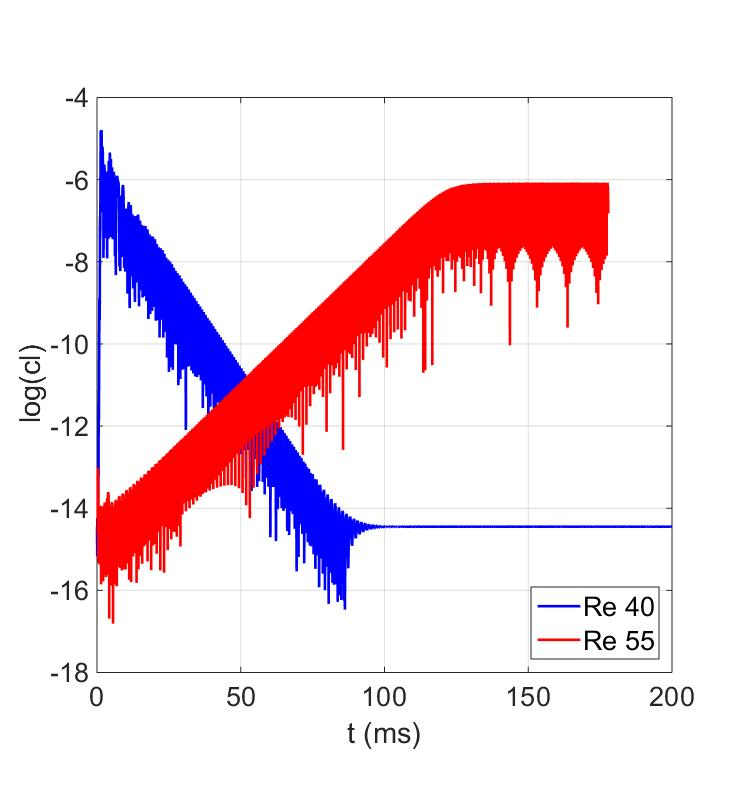
\includegraphics[width=0.49\textwidth]{pic/cl-log.jpg}
	\caption{Lift coeffient histogram for $Re=55$ and $Re=40$.}
	\label{fig:cyl-re40-re55-uns}
\end{figure}

\subsubsection{Eigenvalue analysis}
An eigenvalue analysis is performed for the steady state solution calculated
in NutsCFD. After converging the steady state solver to machine error ($tol=10^{-14}$),
the exact Jacobian matrix based on the 2nd-order spatial accuracy is calculated and
output to file. The sparse matrix is read into Matlab and eigs is used to compute
a subset of the eigenvalues, with the aim of finding the (hopefully one) unstable mode.
To minimize the computational effort, 10 eigenvalues/vectors are computed for
matrices with different shifts of $0$, $i$, $2i$, $3i$, $4i$, $5i$. All the eigenvalues,
60 in total and with some duplicated, are plotted in Fig.~\ref{fig:cyl-re55-eigen-vs-uns}.
It can be seen that there is one eigenvalue that is on the right side of the imaginary axis,
indicating there is one unstable mode. In the meantime, from the time-domain simulation,
one can extract from the lift-coefficient signal that the flow is linearly growing with a
growth rate of 0.123 and oscillating with a circular frequency of $4.94 rad/s$. This
mode is plotted along with the spectrum and it can be seen that this mode also overlaps
with the unstable eigenvalue from the eigenanalysis. 

\begin{figure}[htb]
	\centering   
	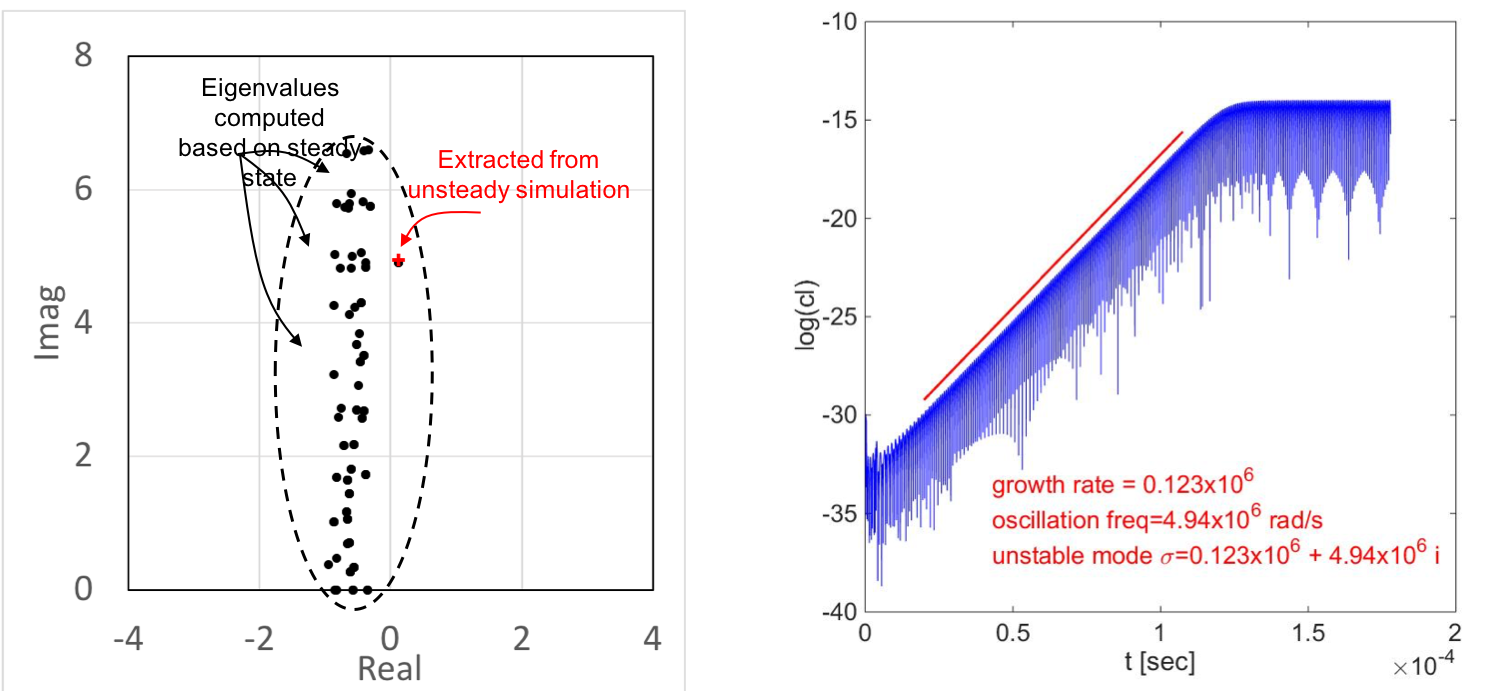
\includegraphics[width=0.9\textwidth]{pic/uns-vs-eigen.png}	
	\caption{Eigenspectrum from the steady state eigenvalue analysis
		compared with the linearly destabiling unsteady simulation for $Re=55$.}
	\label{fig:cyl-re55-eigen-vs-uns}
\end{figure}

The eigenanalysis not only generates the eigenvalues but also the eigenvectors
associated with each eigenvalue. For the unstable mode, the real part of the
density, x/y momentum and energy component of the unstable eigenvector
is shown in Fig.\ref{fig:cyl-re55-eigenmode}.
\begin{figure}[htb]
	\centering   
	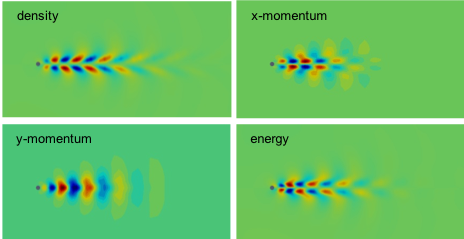
\includegraphics[width=0.98\textwidth]{pic/eigenmode-real.png}	
	\caption{Real part of the density, x/y momentum, energy components
		of the unstable eigenmode for $Re=55$.}
	\label{fig:cyl-re55-eigenmode}
\end{figure}

%
%We use the NutsCFD to compute the steady state laminar flow around the
%circular cylinder for Reynolds number 50, 60 and 75. Eigenvalue analysis is
%performed for each case. The three spectra is shown in Fig.~\ref{fig:cyl}.
%It can be seen that linearly unstable mode start to appear from Re=60.
%The unstable mode at Re=60 is visualized on the right in Fig.~\ref{fig:cyl}
%where our results based on the NutsCFD solver is compared to that
%computed using Nektar++~\cite{cantwell2015nektar++}.
%
%\begin{figure}[htb]
%	\centering   
%	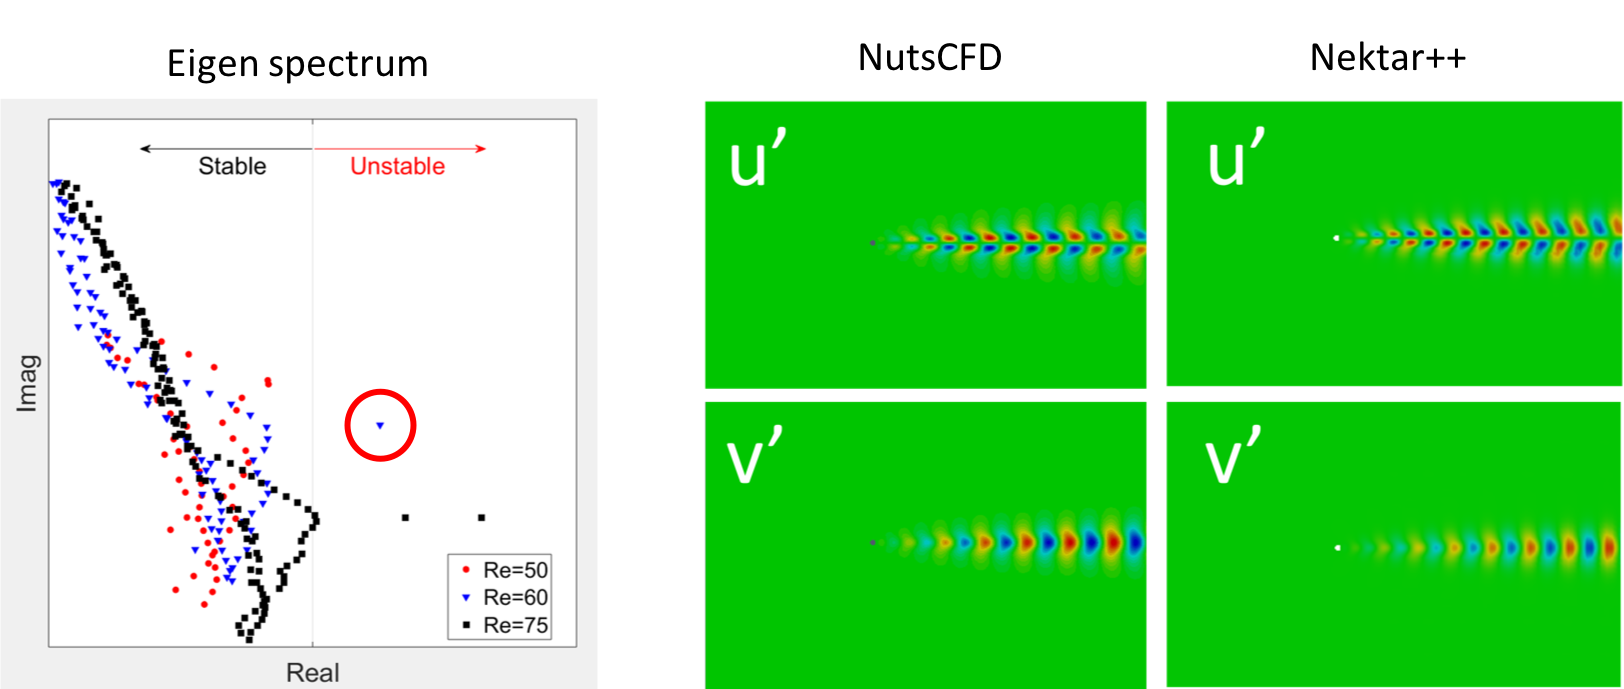
\includegraphics[width=0.99\textwidth]{pic/cyl.png}
%	\caption{Left: spectra computed for the laminar flow around circular cylinder
%		at different Reynolds number; right: x- and y-velocity components
%		of the unstable eigenvector computed by NutsCFD compapred with
%		that with Nektar++.}
%	\label{fig:cyl}
%\end{figure}
%
%\subsection{Transonic buffet around a two-dimensional airfoil (NACA0012)}
%
%\subsubsection{Steady state calculation}
%\subsubsection{Unsteady calculation}
%\subsubsection{Eigenvalue analysis}

\subsection{Transonic flow for a single blade (quasi-3D analysis)}
NutsCFD is used to analyze the performance of the first
stage rotor (NASA Rotor 67) of a two stage transonic fan
designed and tested at the NASA Glenn center~\cite{strazisar1989laser}.
Its design pressure ratio is
1.63, at a mass flow rate of 33.25 kg/sec. 
The NASA Rotor 67 has 22 blades with tip radii of 25.7 cm
and 24.25 cm at the leading and trailing edge, respectively,
and a constant tip clearance of 1.0 mm. The hub to tip radius
ratio is 0.375 at the leading edge (TC = 0.6\% span) and 0.478
at the trailing edge (TC = 0.75\% span). The design rotational
speed is 16,043 RPM, and the tip leading edge speed is 429 m/s
with a tip relative Mach number of 1.38.

\subsection{Compressor performance characteristics}
Steady state analysis is performed for both
the single-passage and whole-annulus
configurations. In order to obtain the steady state
solutions for the whole annulus, which presumably
is identical for each blade passage, we first compute
the steady state solution for one passage with
rotatioal periodicity, and then copy the solution
to the whoe annulus using rotational transformation.
The pressure ratio and efficiency are shown in Fig.~\ref{fig:r67-performance}
which is produced by incrementally raising the back pressure
from the inlet total condition. It can be seen that there is small
difference (mainly efficiency) between the single-passae and
whole-annulus results, which is due to the minor discrepancy
of the spatial discretization at the periodic boundaries for single
passage calculation.

\begin{figure}[htb]
	\centering   
	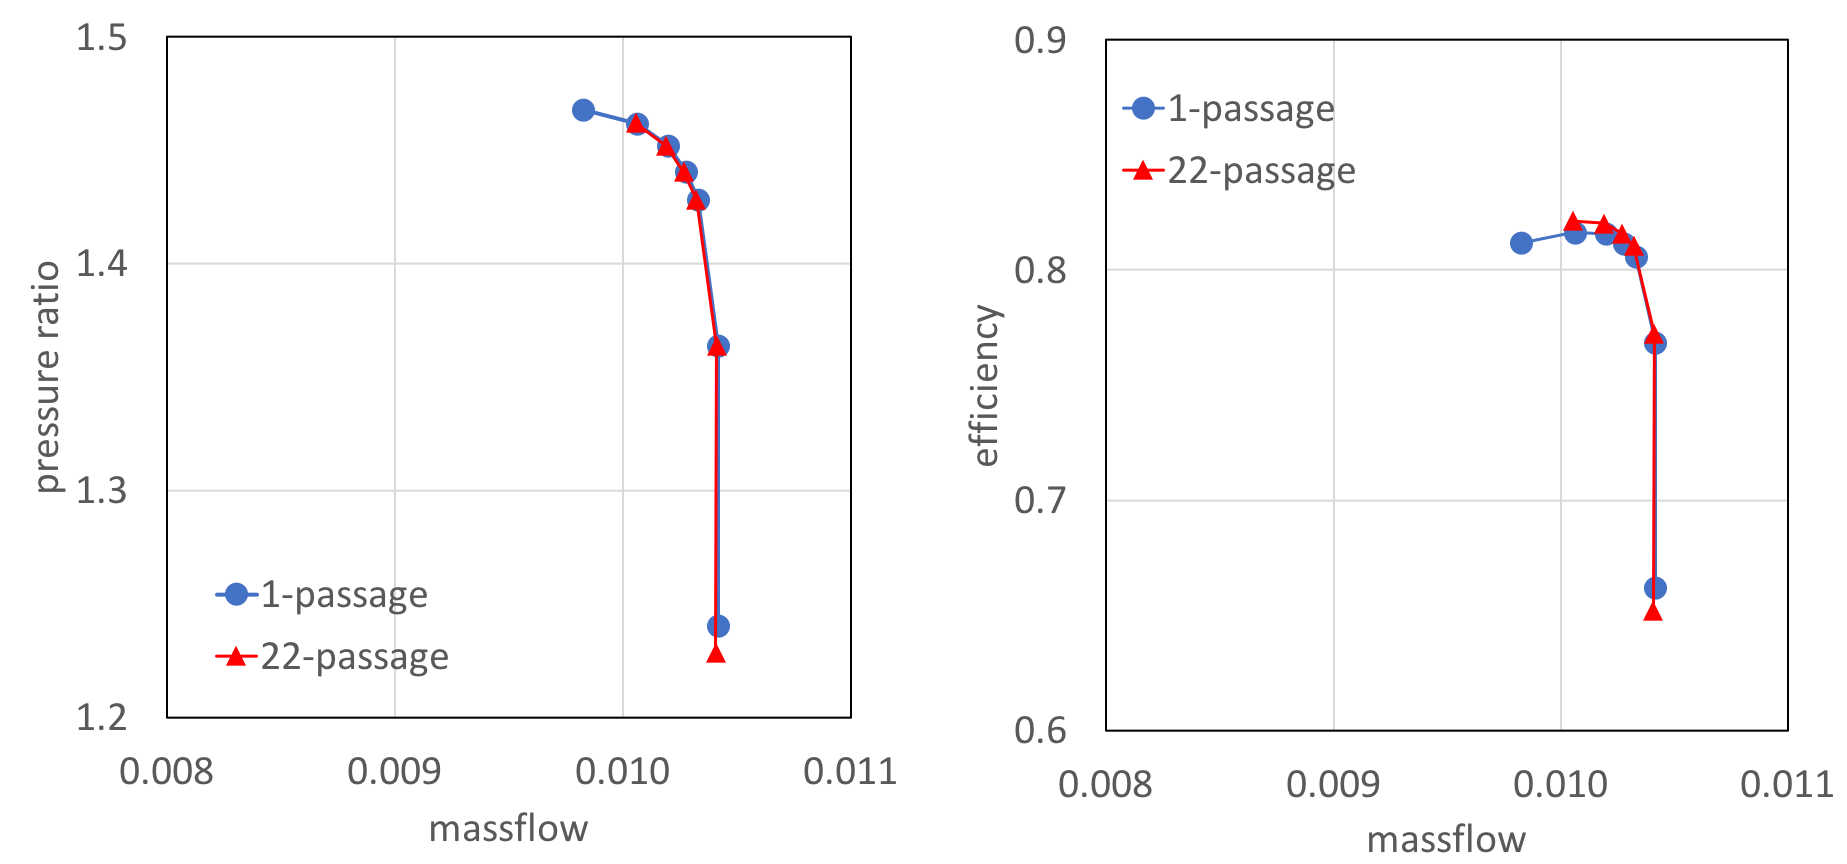
\includegraphics[width=0.9\textwidth]{pic/rotor67-performance.png}
	\caption{Q3D performance for rotor67 at 50\% blade height with either
		single passage or whole annulus (22 passages).}
	\label{fig:r67-performance}
\end{figure}

The flow solution using either single passage or whole annulus
is shown in Fig.~\ref{fig:r67-flow}, which visually shows that
the solutions are not distinguishable.

\begin{figure}[htb]
	\centering   
	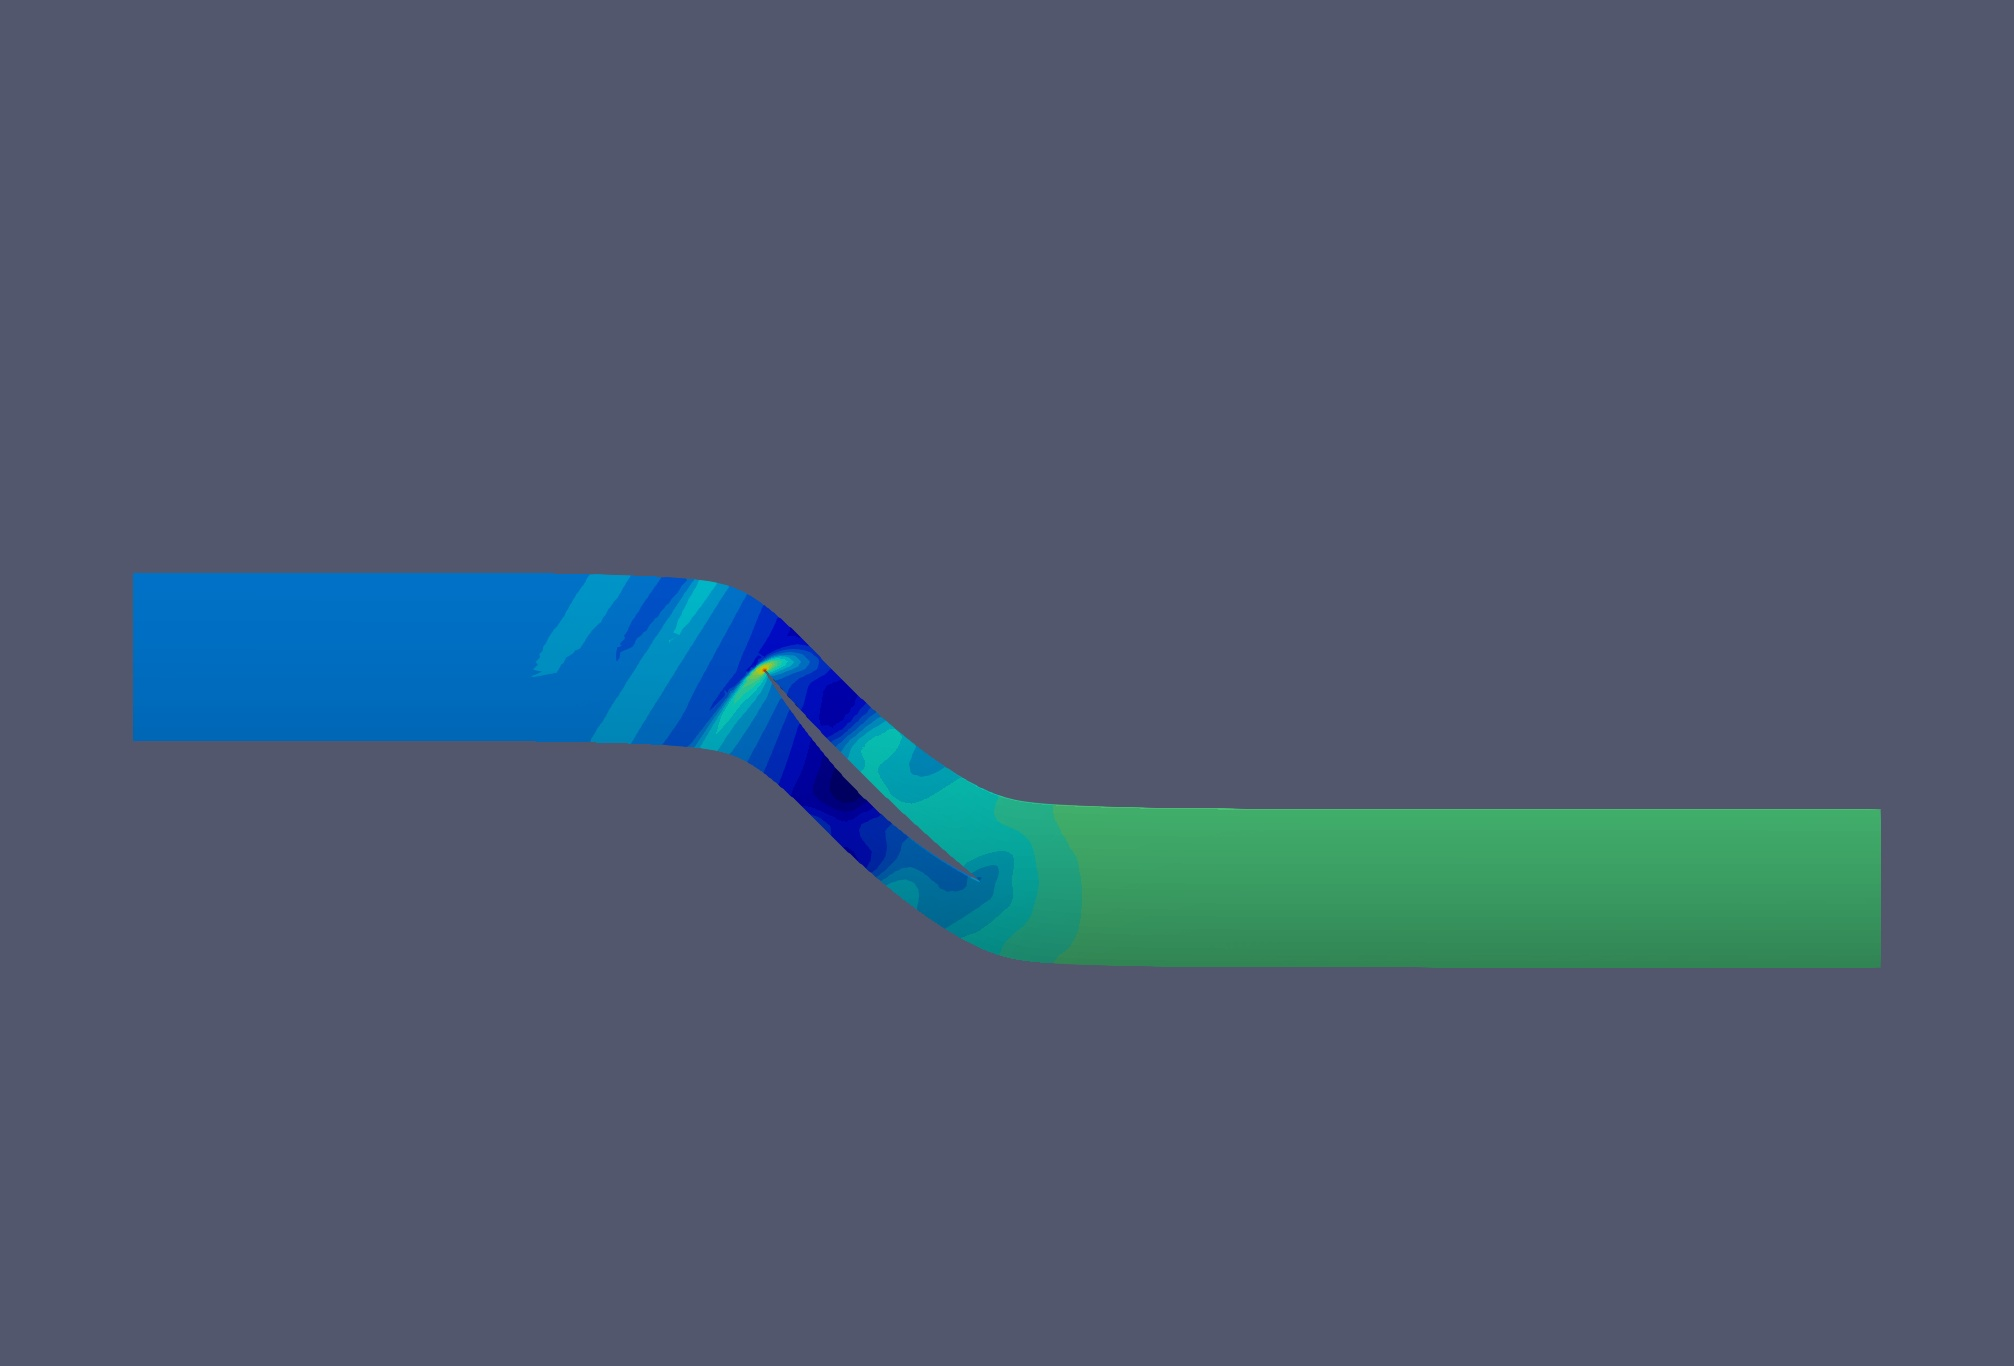
\includegraphics[width=0.45\textwidth]{pic/pressure-1passage.jpeg}
	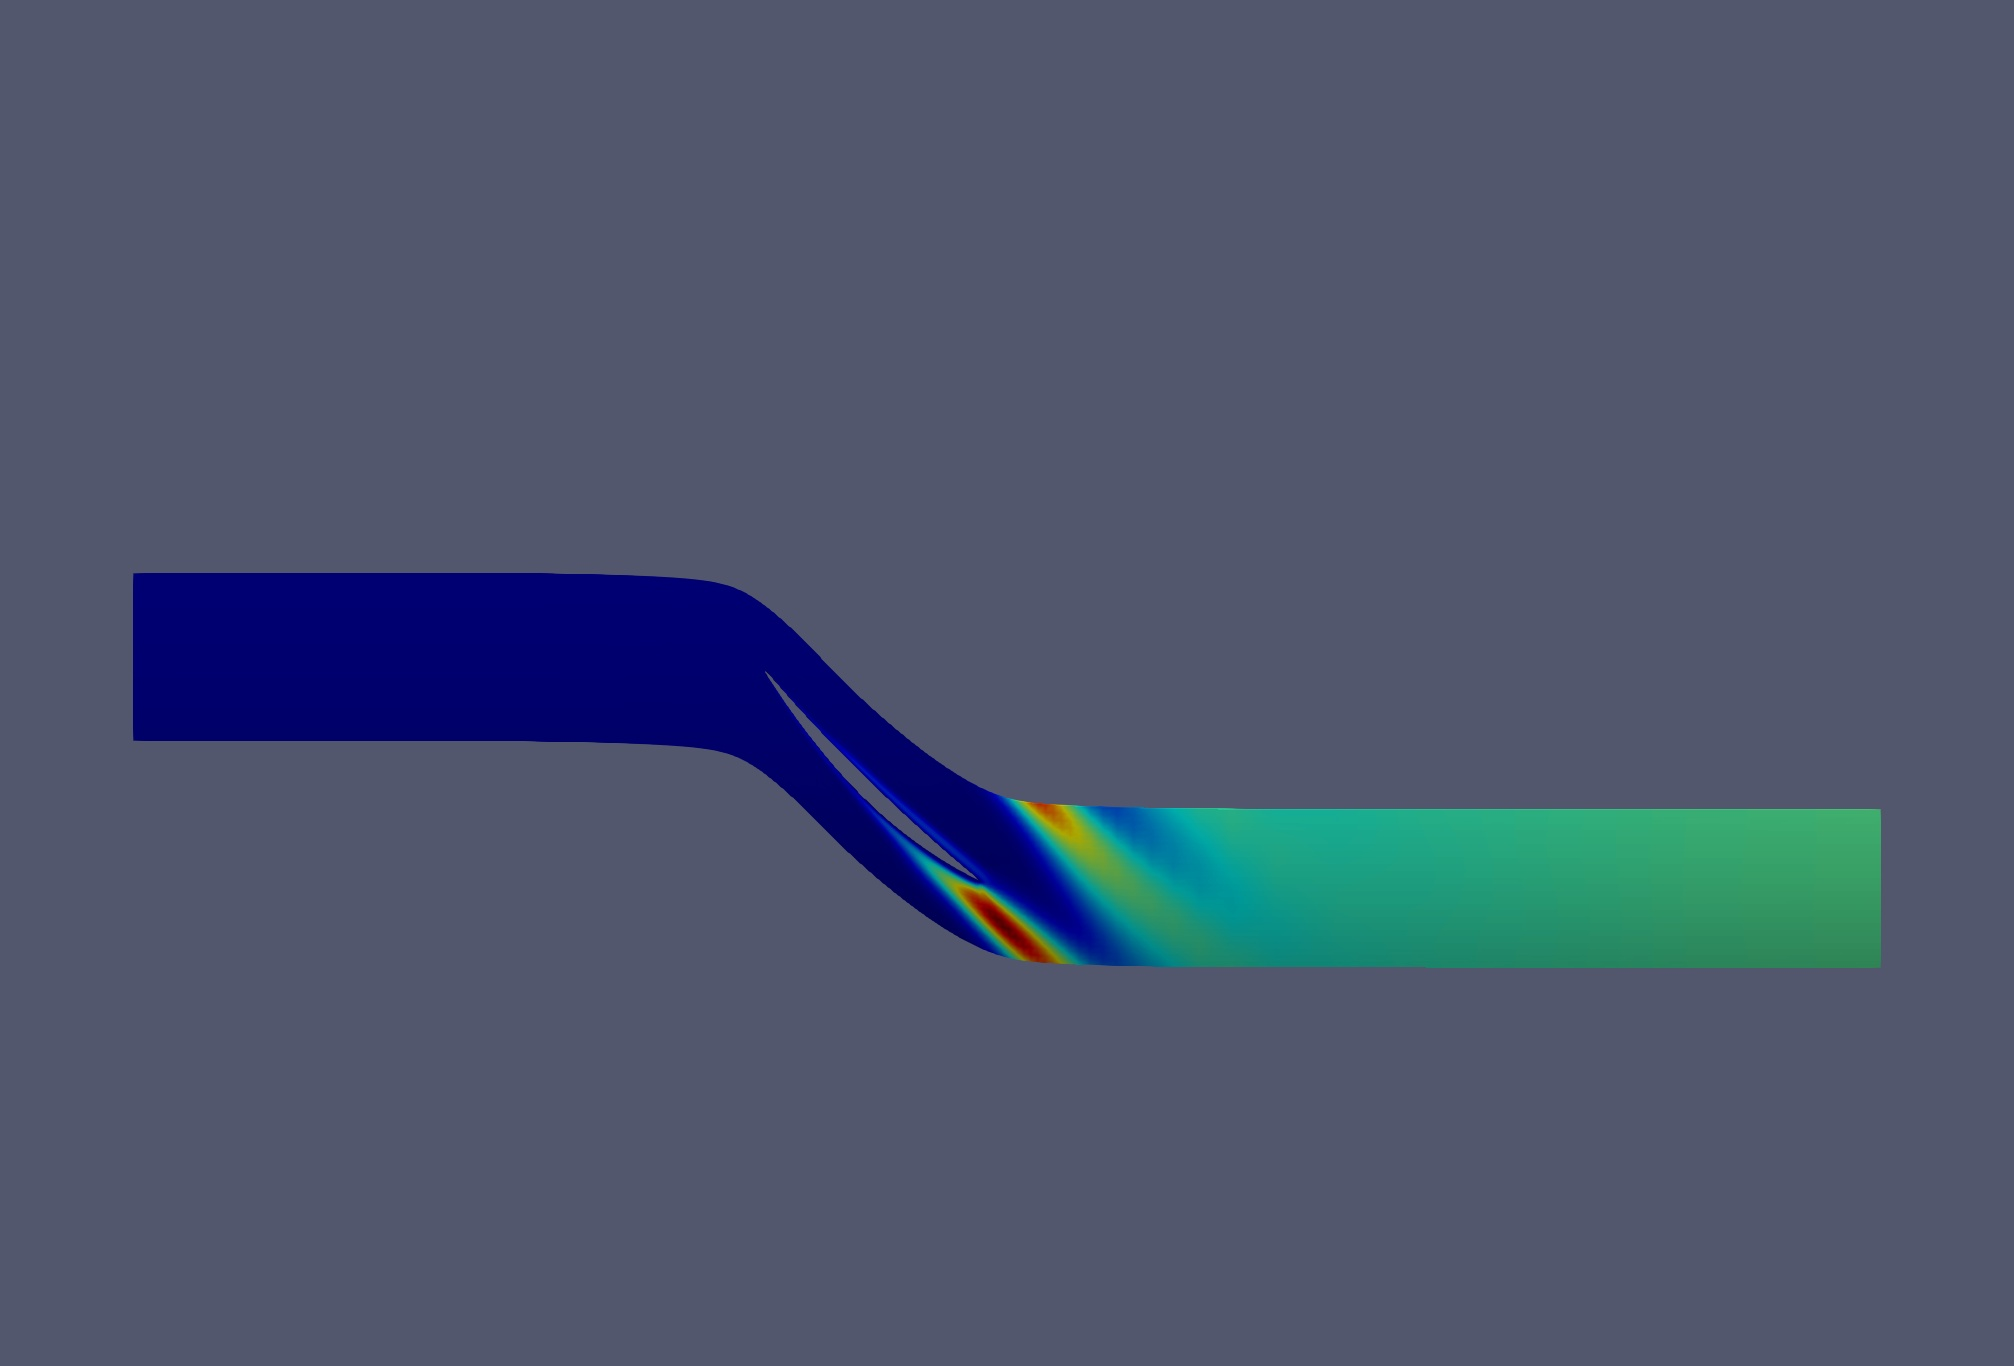
\includegraphics[width=0.45\textwidth]{pic/sa-1passage.jpeg}\\    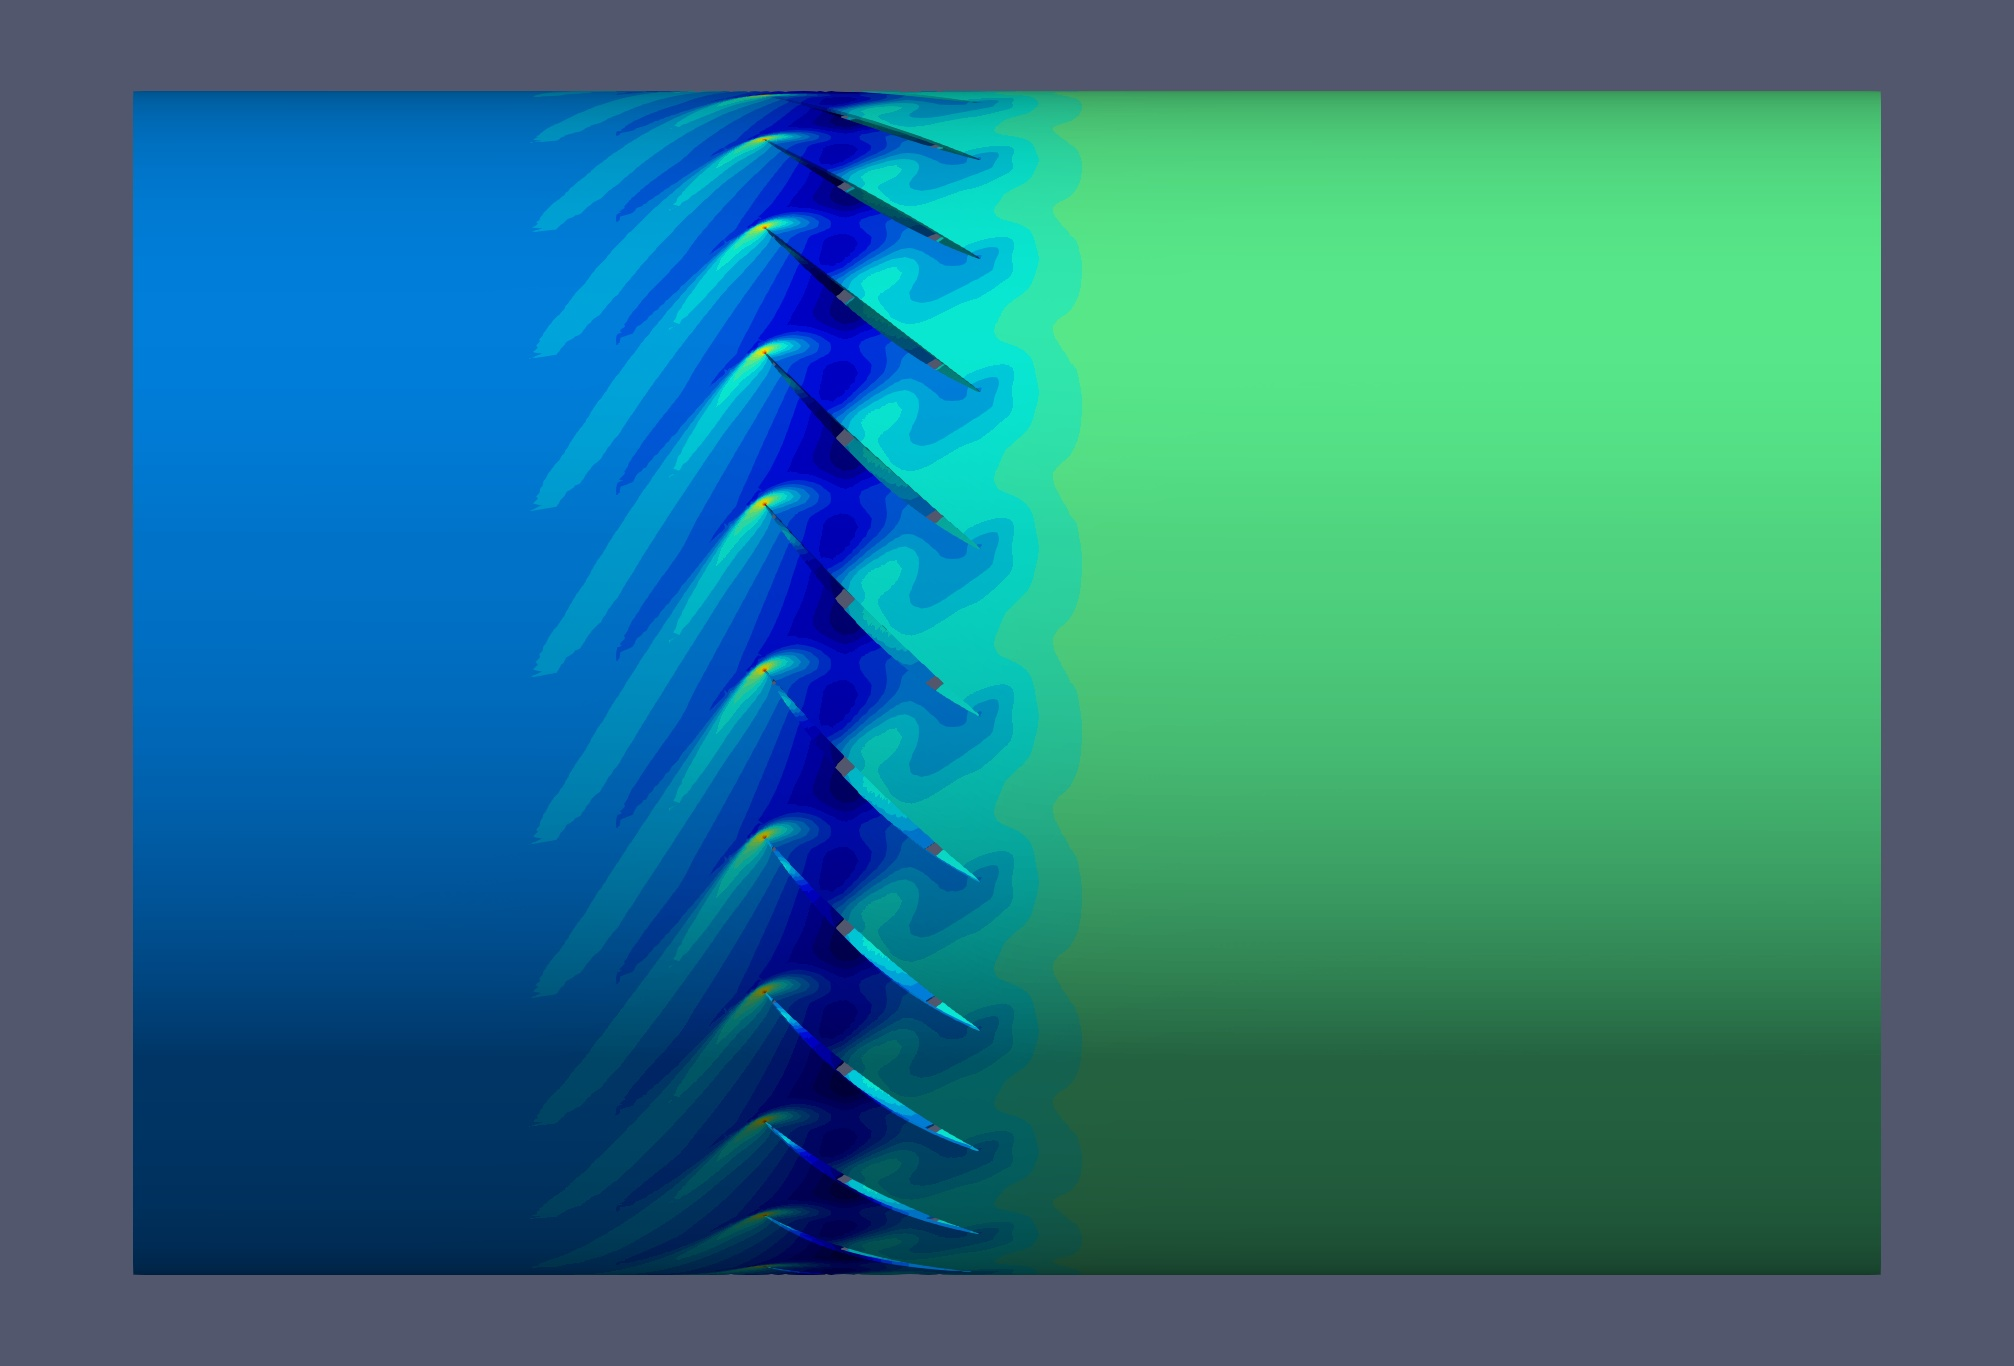
\includegraphics[width=0.45\textwidth]{pic/pressure-22passage.jpeg}
	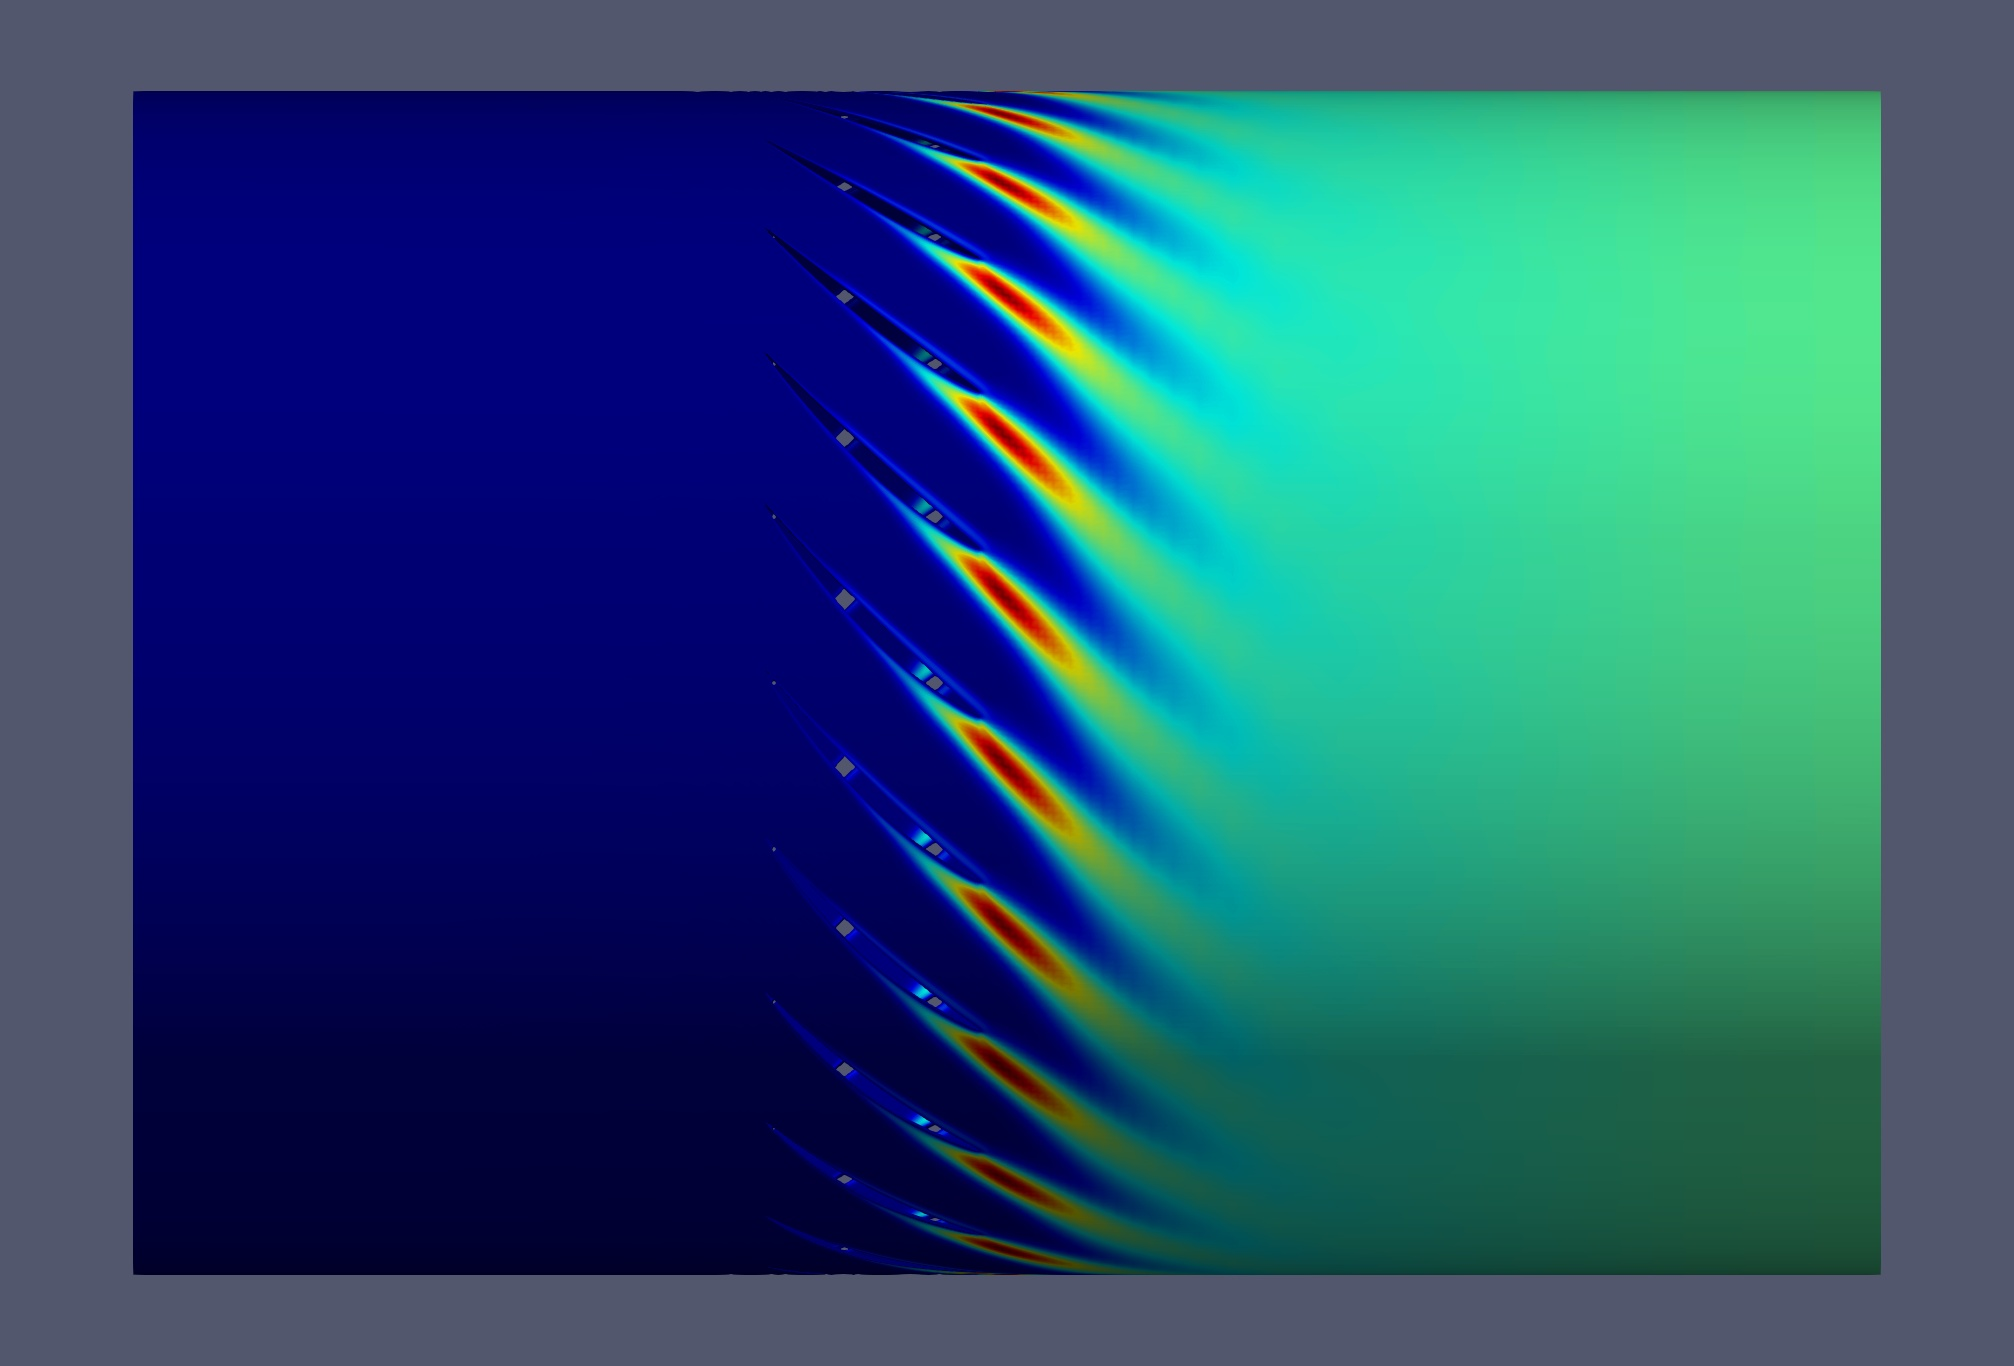
\includegraphics[width=0.45\textwidth]{pic/sa-22passage.jpeg}
	\caption{Pressure (left) and SA variable (right) contours for
	single passage (top) and whole annulus (bottom) calculations.}
	\label{fig:r67-flow}
\end{figure}

\subsection{Eigenvalue analysis}

For each whole-annulus steady state solution, an eigenvalue analysis
is performed using the Jacobian matrix output from the NutsCFD solver
once the steady state calculation has fully converged.
Since the rotational speed for the rotor is 16,043 RPM, the Jacobian
matrix is scaled by a factor of $1/(2\pi \times 16,043 / 60)\approx 1/1680$,
so that all frequencies involved in this computation is reduced by the
rotor angular frequency. This is done due to the pre-knowledge that
rotating stall cells move with speed of the same order of magnitude.

Shown in Fig.~\ref{fig:r67-eigen-18kpa} is a subset of the eigenvalues
that are near the imaginary axis, which presumally are most likely to
be unstable. The eigs function in Matlab is used with various
imaginery shifts to compute interior eigenvalues. The ones that
are suspecious of crossing the imaginery axis are shown. A zoomed
view of the eigenvalues reveals that there are a total of five that
have positive real parts, i.e., unstable. The pressure component
of the eigenvector corresponding to the 3rd eigenvalue is
visualized to the right of Fig.~\ref{fig:r67-eigen-18kpa}. The
circumferential synchronized shock oscillation can be easily spotted.
Eigenvectors of other unstable mode are similar, except with different
circumferential variation, which can further be attributed to different
nodal diameters, which varies from 5 to 9, continuously, from eigenvalues
1 to 5.



\begin{figure}[htb]
	\centering   
	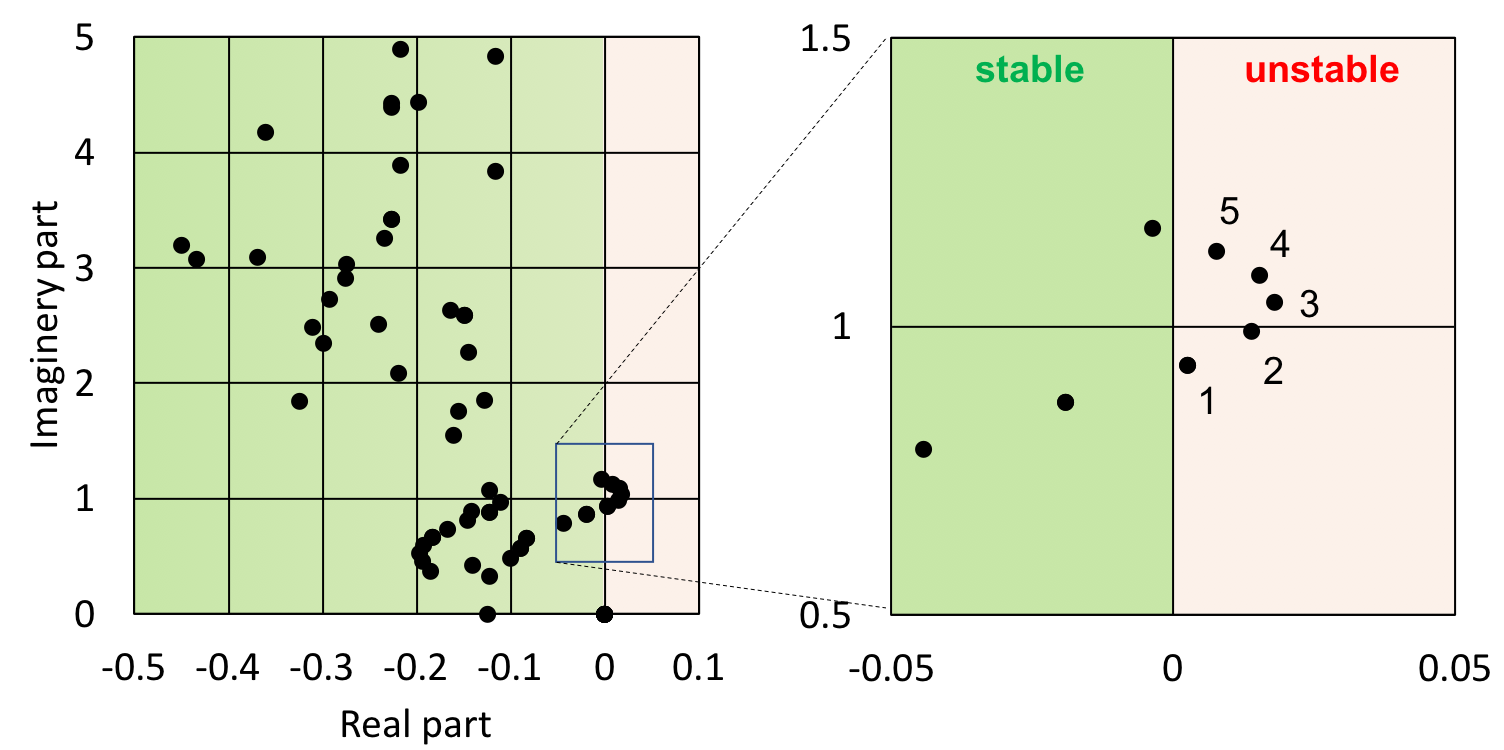
\includegraphics[width=\textwidth]{pic/rotor67-2d-eigenvalue-18kpa.png}
	\caption{18kpa eigenvalue.}
	\label{fig:r67-eigen-18kpa}
\end{figure}


\begin{figure}[htb]
	\centering   
	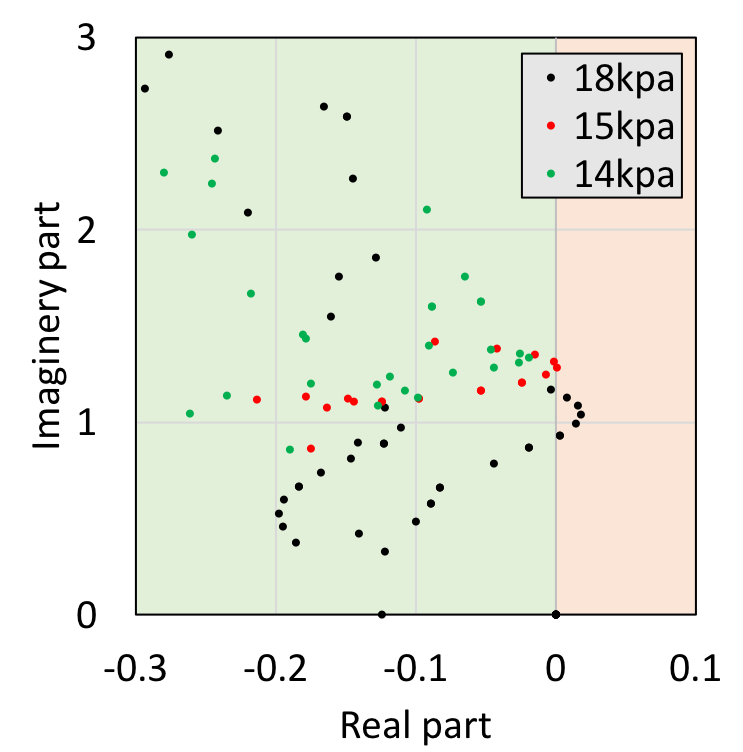
\includegraphics[width=.5\textwidth]{pic/eigenvalue-14-18kpa.png}
	\caption{18kpa eigenvalue.}
	\label{fig:r67-eigen-14-18kpa}
\end{figure}



Nodal diamater for different eigenmodes?

\section{Conclusion}
\label{conclusion}

\section*{Acknowledgements}

\bibliography{xu}

\end{document}
